% Figure: the work plan of the proposal as a bar chart over twelve months.
% Standalone TikZ source. The colors match the figures of the manuscript.
\documentclass[tikz,border=2pt]{standalone}
\usetikzlibrary{arrows.meta,calc,shapes.geometric}

\definecolor{ink}{HTML}{0B0B0B}
\definecolor{inksoft}{HTML}{52514E}
\definecolor{gridgray}{HTML}{E1E0D9}
\definecolor{axisgray}{HTML}{C3C2B7}
\definecolor{barfill}{HTML}{CDE2FB}
\definecolor{barborder}{HTML}{1C5CAB}
\definecolor{milestone}{HTML}{EB6834}

\begin{document}
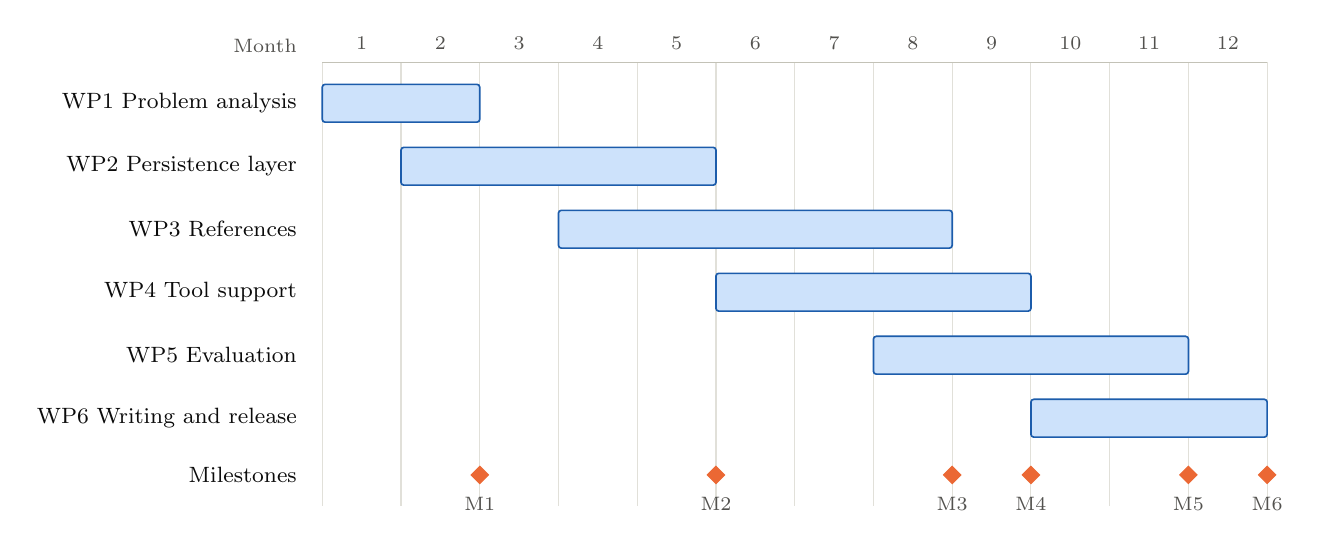
\begin{tikzpicture}[
  x=10mm, y=8mm, font=\footnotesize,
  bar/.style={fill=barfill, draw=barborder, line width=0.6pt, rounded corners=1pt},
  wp/.style={anchor=east, text=ink},
  month/.style={anchor=south, text=inksoft, font=\scriptsize},
  gridline/.style={draw=gridgray, line width=0.4pt},
  mstone/.style={diamond, fill=milestone, draw=milestone, inner sep=1.6pt},
  mlabel/.style={anchor=north, text=inksoft, font=\scriptsize}
]

\foreach \m in {0,1,...,12} {\draw[gridline] (\m,0.15) -- (\m,-6.9);}
\foreach \m in {1,...,12} {\node[month] at (\m-0.5,0.2) {\m};}
\node[wp, text=inksoft, font=\scriptsize] at (-0.2,0.42) {Month};
\draw[draw=axisgray, line width=0.5pt] (0,0.15) -- (12,0.15);

\node[wp] at (-0.2,-0.5) {WP1 Problem analysis};
\fill[bar] (0,-0.8) rectangle (2,-0.2);
\node[wp] at (-0.2,-1.5) {WP2 Persistence layer};
\fill[bar] (1,-1.8) rectangle (5,-1.2);
\node[wp] at (-0.2,-2.5) {WP3 References};
\fill[bar] (3,-2.8) rectangle (8,-2.2);
\node[wp] at (-0.2,-3.5) {WP4 Tool support};
\fill[bar] (5,-3.8) rectangle (9,-3.2);
\node[wp] at (-0.2,-4.5) {WP5 Evaluation};
\fill[bar] (7,-4.8) rectangle (11,-4.2);
\node[wp] at (-0.2,-5.5) {WP6 Writing and release};
\fill[bar] (9,-5.8) rectangle (12,-5.2);

\node[wp] at (-0.2,-6.4) {Milestones};
\foreach \m/\name in {2/M1, 5/M2, 8/M3, 9/M4, 11/M5, 12/M6} {
  \node[mstone] at (\m,-6.4) {};
  \node[mlabel] at (\m,-6.6) {\name};
}
\end{tikzpicture}
\end{document}
